\documentclass[12pt]{article}
\usepackage{amsfonts, epsfig}
\usepackage[authoryear]{natbib}
\usepackage{graphicx}
\usepackage{fancyhdr}
\pagestyle{fancy}
\lfoot{\texttt{com30127.github.io}}
\lhead{Computational Neuroscience - 01.2 Synapses  - Conor}
\begin{document}

\section*{Synapses}

In the previous section we discussed action potentials, the voltage
pulses that travel along axons and carry signals from neuron to
neuron. What we didn't discuss was how the signals got from the axon
of one neuron to the dendrite of the next. The answer is synapses. 

In discussing the action potential we mentioned that it is a largely
stereotypical signal, the action potentials from a neuron all have
roughly the same amplitude and shape. The synapses, in contrast, are
very variable; they have different strengths, the strengths can change
over time. Beyond these variations in strength, synapses can have very
different dynamics, with differences in the time course of how the
synapse responds to a spike, or in how the synapse responds to spikes
coming in quick succession.

The complicated and variable behaviours of synapses are possible
because synapses do not simply connect the axon to the dendrite, they
are not simply holes or pores through which ions flow. In fact, there
are synapses, called \textsl{gap junctions} that are like that, these
gap junctions are the only synapses in some simple creatures like
jellyfish and are found in the mammalian brain. However, the synapses
we usually have in mind are \textsl{chemical synapses} in which the
signal transfer from \textsl{pre-synaptic} axon to
\textsl{post-synaptic} dendrite involves a complex chemical cascade.


\subsection*{Chemical synapses} 

\begin{figure}[tbhp]
  \begin{center}
    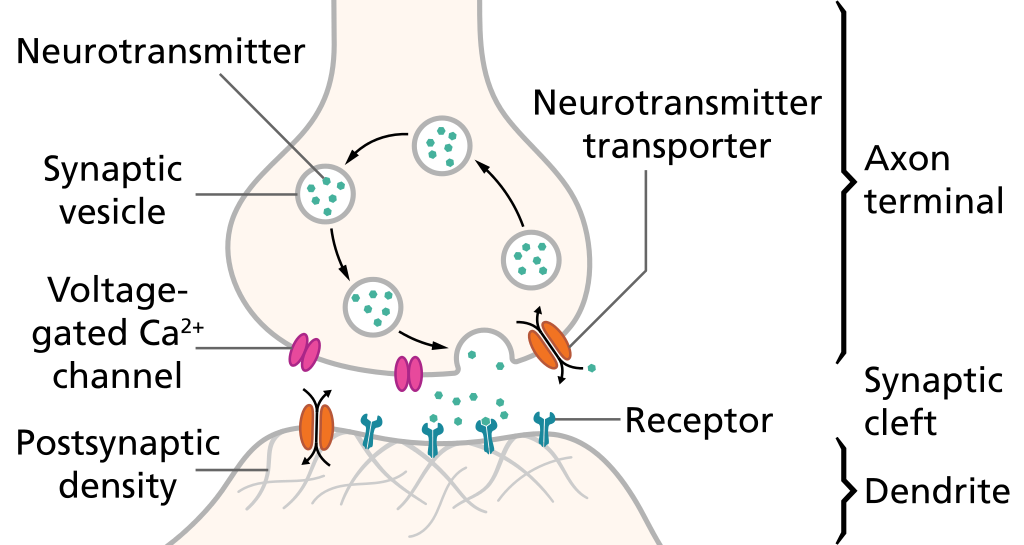
\includegraphics[width=8cm]{synapse.png}
    \end{center}
  \caption{\textbf{A diagram of a synapse}; this cartoon shows the
    main parts of the synapse; the axon of the pre-synaptic neuron is
    coming in from the top, the dendrite of the post-synaptic neuron
    is leaving through the bottom. Figure from
    \texttt{wikipedia}\label{fig_synapse}}
\end{figure}

In Fig.~\ref{fig_synapse} is a cartoon of a synapse. The first thing
to note is that the dendrite and axon don't actually touch; there is a
little gap, called the \textsl{synaptic cleft} between the two. Of
course, the axon and dendrite are held together by glial cells, cells
which also surround the cleft and keep everything in place. In
important thing though, is that the charge doesn't flow directly from dendrite to axon.

When a spike arrives at the synapse it kicks off a chain of
events. The sudden change in voltage opens channels in the membrane of
the synapse which allow calcium to flow into the \textsl{terminal button}, the part of the synapse on the axon side of the cleft; it is an
amazing property of neurons that they contain ion-specific
channels. The calcium flows into the synapses and, by way of
complicated chemical reactions, this causes some little spheres called
\textsl{vesicles} to fuse with the wall of the cleft and burst
releasing some very specialized molecules called
\textsl{neurotransmitters} into the cleft. These neurotransmitters, in
turn, bind with channels on the opposite face of the cleft, that is,
with channels in the membrane of the post-synaptic dendrite.

These channels, in turn, in response to binding with the
neurotransmitter, open and depending on the type of synapse, they
either allow ions to flow into, or out of, the dendrite, either
increasing its voltage, or decreasing it. In other words, before
looking at all the other variations, there are two main types of
chemical synapses, \textsl{excitatory} synapses, that increase the
voltage of the post-synaptic neurons and \textsl{inhibitory} synapses
that decrease it.

Each type of synapse has different channels in the dendritic face of
the cleft and different neurotransmitter which binds to these
channels. In an excitatory synapses these channels allow sodium ions
into the cell; since sodium ions are positive ions this increases the
charge inside the cell. Depending on exactly what type of inhibitory
synapse it is, in an inhibitory synapse the channels either allow
chlorine ions into the dendrite, chlorine ions are negative so this
decreases the voltage, or they allow potassium ions out of the cell,
potassium ions are positive, so again this decreases the voltage.

The channels open because they have bonded with the neurotransmitter;
they are called \textsl{ligand-gated channels}; a ligand is a molecule
that binds to things and so these are channels that act as gates,
sometimes allowing ions through and sometimes not and they do so
depending on whether or not they are bound to a ligand. This is in
contrast with the \textsl{voltage-gated channels} that open to let the
calcium in, these open and close depending on voltage and, we will
see, voltage gated channels are also important in understanding how
spiking happens. The binding between ligand and ligand-gated channel
is quite loose and the molecules are bathed in a warm fluid; random
Brownian movements will unbind the ligand allowing the channel to
close. The timescale for this unbinding is different for different
channels; for typical excitatory synapses it is of the order of tens
of milliseconds. The neurotransmitter in the cleft is also cleared
away by little pumps; the reuptake pumps, and is repackaged into
vesicles ready for the arrival of later spikes.

The final part of this story is the dendrite itself; consider first
the situation with a excitatory neuron. The current flow into the
neuron increases the voltage, this ramps up as more and more
ligand-gated channels open before decaying away again as they
close. The resulting positive pulse is called an \textsl{excitatory
  post-synaptic potential} or EPSP. For an inhibitory synapse the
pulse is negative and is called an \textsl{inhibitory post-synaptic
  potential} or IPSP. Example PSPs are showing Fig.~\ref{fig_psp}.


\begin{figure}[tbhp]
  \begin{center}
    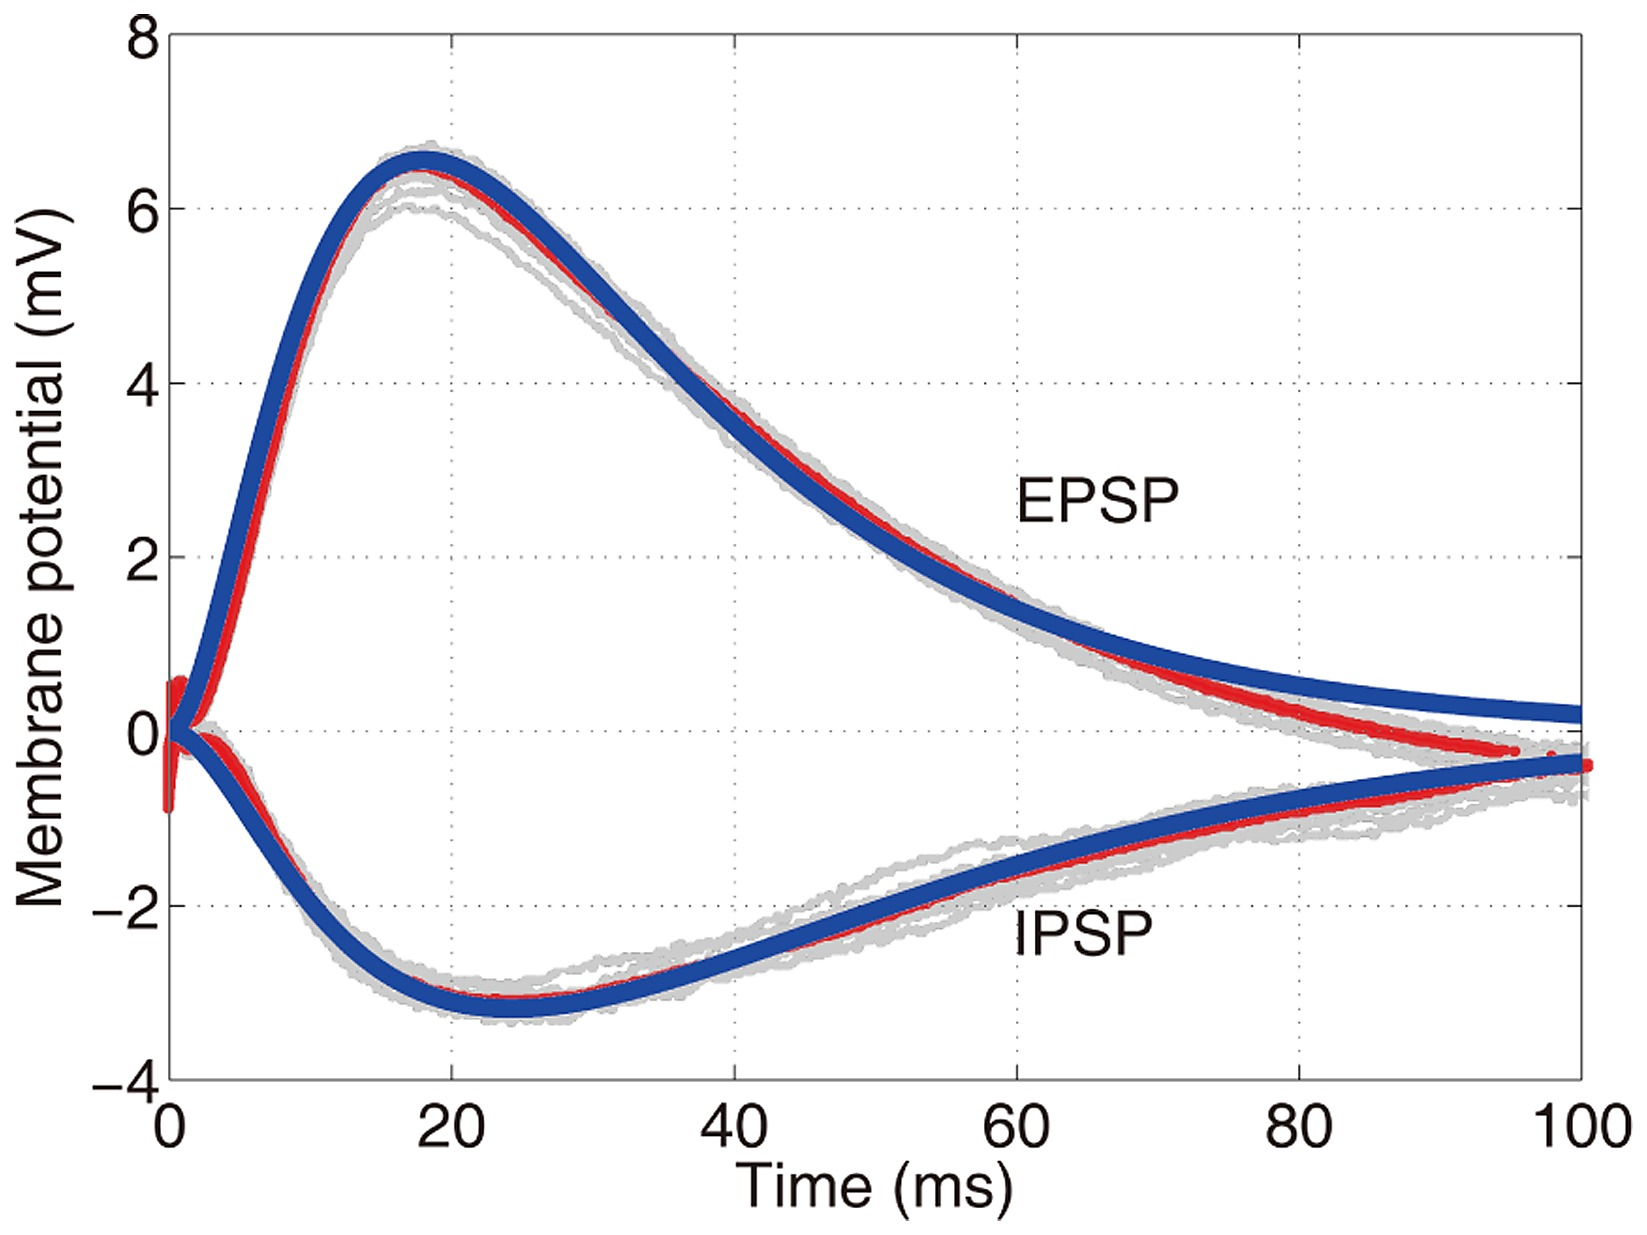
\includegraphics[width=8cm]{psp.jpg}
    \end{center}
  \caption{\textbf{Some PSPs}; the grey lines are recordings for
    individual PSPs with the red lines giving averages and blue lines
    demonstrate a model; we will look at simple models of PSPs
    later. Figure from \cite{ZhouEtAl2013}\label{fig_psp}}
\end{figure}

In general dendrites lack the voltage-gated channels needed for action
potentials and the PSPs in dendrites propagate passively towards the
axon. In general dendrites are shorter than axons and thicker, so this
conductance allows the change in voltage at the dendrite to propagate
in to the soma. Even in the soma, where there are voltage gates
channels an individual EPSP won't change the voltage enough to cause a
spike. However, if lots of PSPs arrive at around the same time, the
voltage in the soma will increase until it reaches a tipping point,
around -55 mV is typical value of where this tipping point is. At the tipping point
the opening of voltage-gated channels will cause a spike, usually at
the point the axon joins the soma, and this spike will head off down
the axon.

\section{Summary}

Here we described synapses: this is a complicated story we will go
through again. When the spike arrives at the synapse some of the
vesicles, little bags of neurotransmitter, fuse to the membrane of the
synapse closest to the dendrite and burst, emptying neurotransmitter
into the synaptic cleft. This, in turn, causes channels to open in the
dendrite, changing the potential there. This change in potential, a
PSP, flows into the soma causing a small change in the potential in
the soma. If these small changes add up to push the soma potential to
a threshold, the neuron spikes, sending out an action potential along
the axon.


\bibliographystyle{plain}
\bibliography{../../misc/references}{}


\end{document}

